\section{Parameter Analysis}
\label{params}
In order to analyse the system in more depth, it is possible to plot all parameters for different values, and to see the effect that each of them have on maximum $x$ displacement, maximum $y$ displacement and also the trajectory of the particle as it falls ($x$ and $y$ displacement). This allows for irrelevant parameters to be found, and ideal values for these parameters to be found. \newline \newline
\noindent Each of these simulations are run with the same initial conditions:

\begin{itemize}
\item $u = 0$
\item $v = 0$
\item $\omega = 0$
\item $\theta = 1$
\item $ x = 0$
\item $ y = 0$
\end{itemize}


\subsection{$k{\perp}$ Analysis}
Running the simulation for various values of $k{\perp}$ gives Figures \ref{fig:kpermax} and \ref{fig:kper_xy}. The values chosen are between 0 and 10, and 20 different simulations are run. This also causes an increase in $k_{\parallel}$, as they are directly proportional to each other. 
\begin{figure}[H]
	\centering
	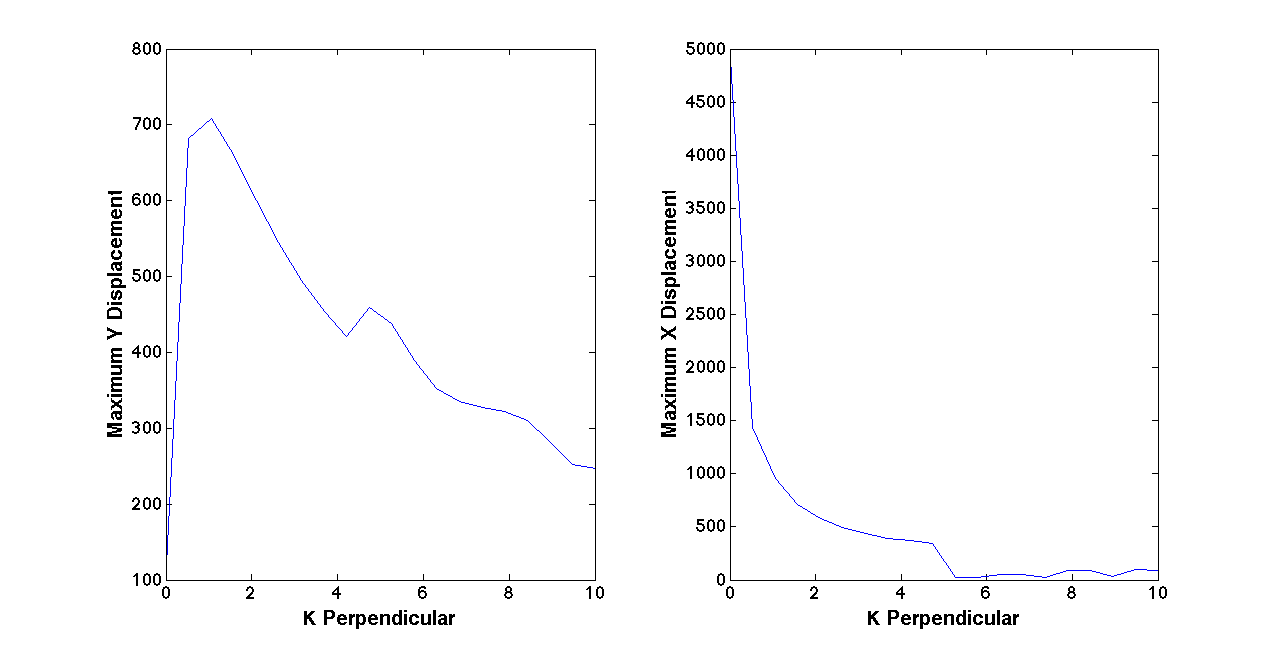
\includegraphics[width=1\textwidth, height=2.5in]{Motion_Graphs/kper_max.png}
	\caption{Plot of maximum $y$ displacement (left) and $x$ displacement (right) against $k{\perp}$ between 0 and 10. Both have a negative gradient, with the $x$ displacement decreasing exponentially.}\label{fig:kpermax}
\end{figure}

\noindent As can be seen in Figure \ref{fig:kpermax}, as the perpendicular and parallel friction increases, the absolute maximum of the displacement along both axis decreases, with the $x$ values reaching a near constant value at around 100 metres. The $y$ also decreases exponentially, beginning to settle at around 300 to 400 metres. 

\begin{figure}[H]
	\centering
	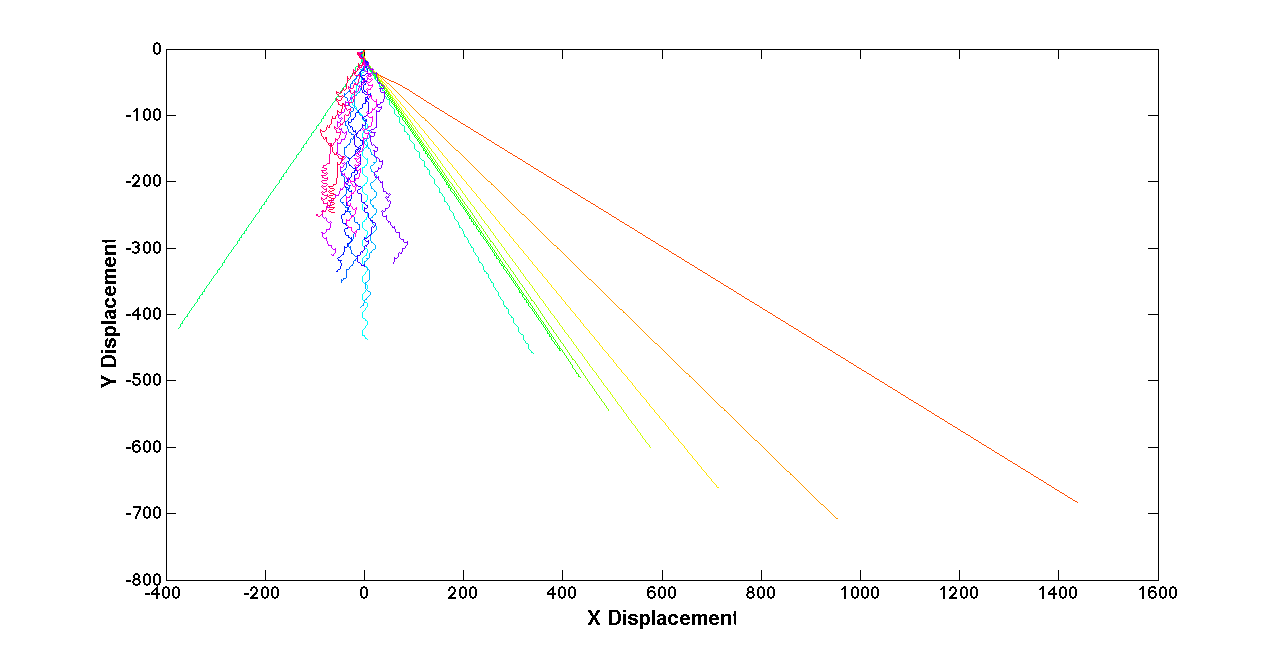
\includegraphics[width=1\linewidth, height=2.5in]{Motion_Graphs/kper_xy.png}
	\caption{Plot showing the trajectory of the leaf as the simulation runs, for 20 values of $k{\perp}$ between 0 and 10. }\label{fig:kper_xy}
\end{figure}

\noindent Figure \ref{fig:kper_xy} shows the trajectory of the leaf as $k{\perp}$ is increased. Below a value of 50, the leaf travels more diagonally, and as it increases above 50, the trajectory of the leaf becomes more oscillatory, as would be expected in this system.

\subsection{Ratio of Density of Air to Density of Leaf $\rho$}
$\rho$ is the ratio of the density of the fluid  the leaf is flowing through to that of the leaf \cite{leaf}. In order to find a suitable value for this, different values (between 0 and 1) were selected, and simulations were run to see the results of the modifications (Figures \ref{fig:rhomax} and \ref{fig:rho_xy}).
\begin{figure}[H]
	\centering
	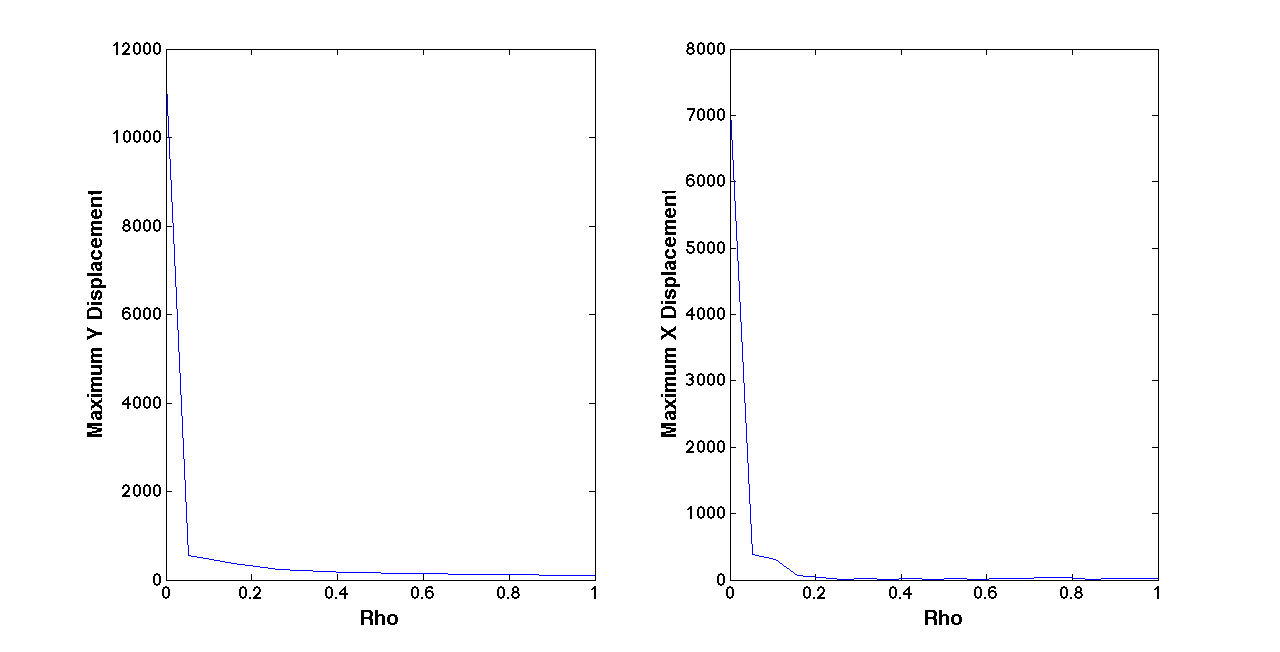
\includegraphics[width=1\textwidth, height=2.5in]{Motion_Graphs/rho_max.png}
	\caption{Plot of maximum $y$ displacement (left) and $x$ displacement (right) against $\rho $ between 0 and 1. Both decrease linearly up until $\rho \approx 0.1 $.}\label{fig:rhomax}
\end{figure}
\noindent As can be seen from Figure \ref{fig:rhomax}, between 0 and 0.1 has a sharp decline in both cases. As it gets to around 0.1 it has a sharp change in gradient, the maximum displacements in both directions level out after 0.2, at a value of around 15 metres in the $x$ displacement case, and just above 100 metres in the $y$ displacement case.


\begin{figure}[H]
	\centering
	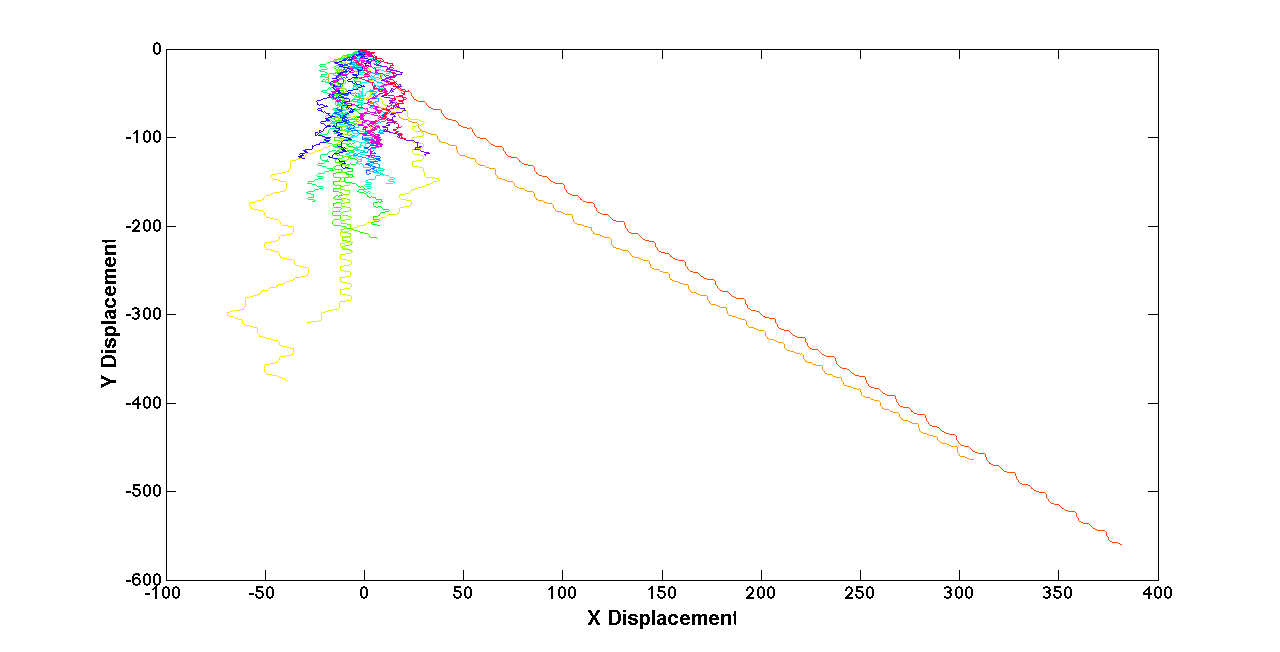
\includegraphics[width=1\linewidth, height=2.5in]{Motion_Graphs/rho_xy.png}
	\caption{Plot showing the trajectory of the leaf as the simulation runs, for 20 values of $\rho$ between 0 and 1. }\label{fig:rho_xy}
\end{figure}

\noindent Figure \ref{fig:rho_xy} shows how $\rho$ affects the trajectory of the leaf. It can be seen that when $\rho < 0.1$ the leaf reaches very large $x$ and $y$ displacements. Higher values of $\rho$ create more believable oscillatory motion. 

\subsection{Ratio between $k{\perp}$ and K-Parallel, f}

f is a division factor applied to $k_{\perp}$ to calculate $k_{\parallel}$. In order to test different $k_{\parallel}$ values independent of the $k{\perp}$ values, a range of values (between 0 and 100) are used. As f increases, $k_{\parallel}$ decreases. 

\begin{figure}[H]
	\centering
	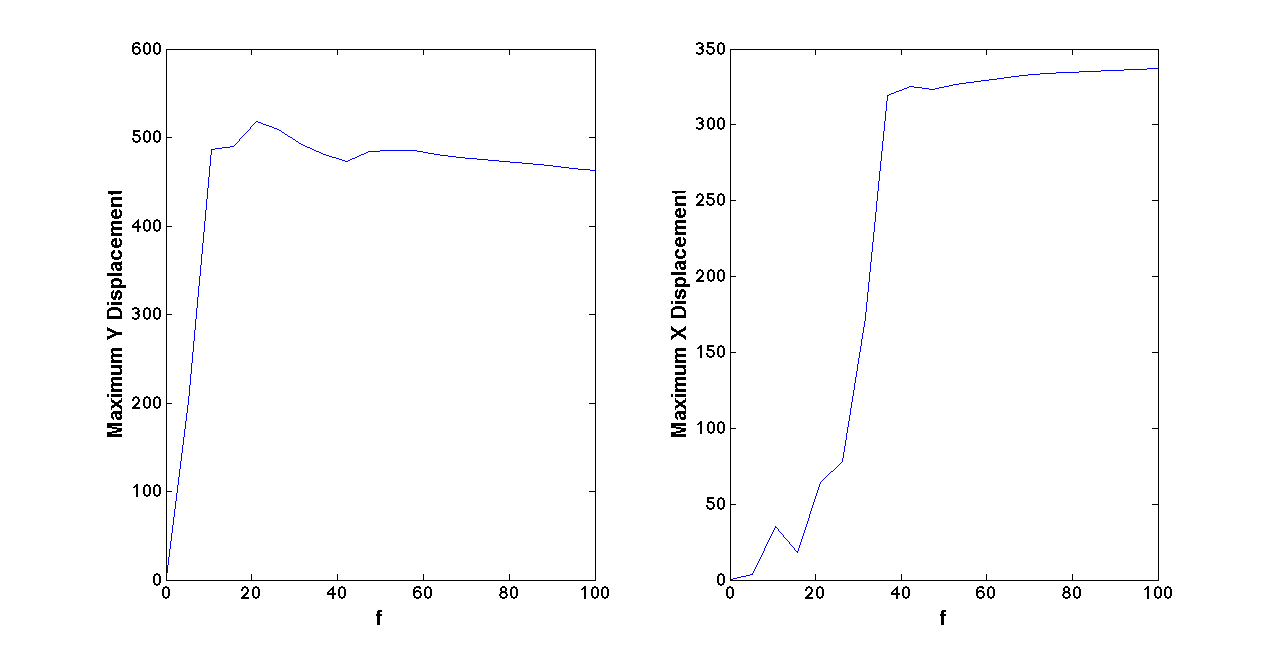
\includegraphics[width=1\textwidth, height=2.5in]{Motion_Graphs/f_max.png}
	\caption{Plot of the maximum $y$ displacement (left) and maximum $x$ displacement (right) against f (the division factor between $k{\perp}$ and $k_{\parallel}$) for values between 0 and 100. }\label{fig:fmax}
\end{figure}

\noindent As can be seen from Figure \ref{fig:fmax}, as f increases from 0 to 15 there is a sharp increase in the maximum $y$ displacement. As it reaches 15, it begins to level out at a value between 450 and 500 metres. The maximum $x$ displacement increases until it reaches around 320 metres, where f is at a value of 40, and it levels out.

\begin{figure}[H]
	\centering
	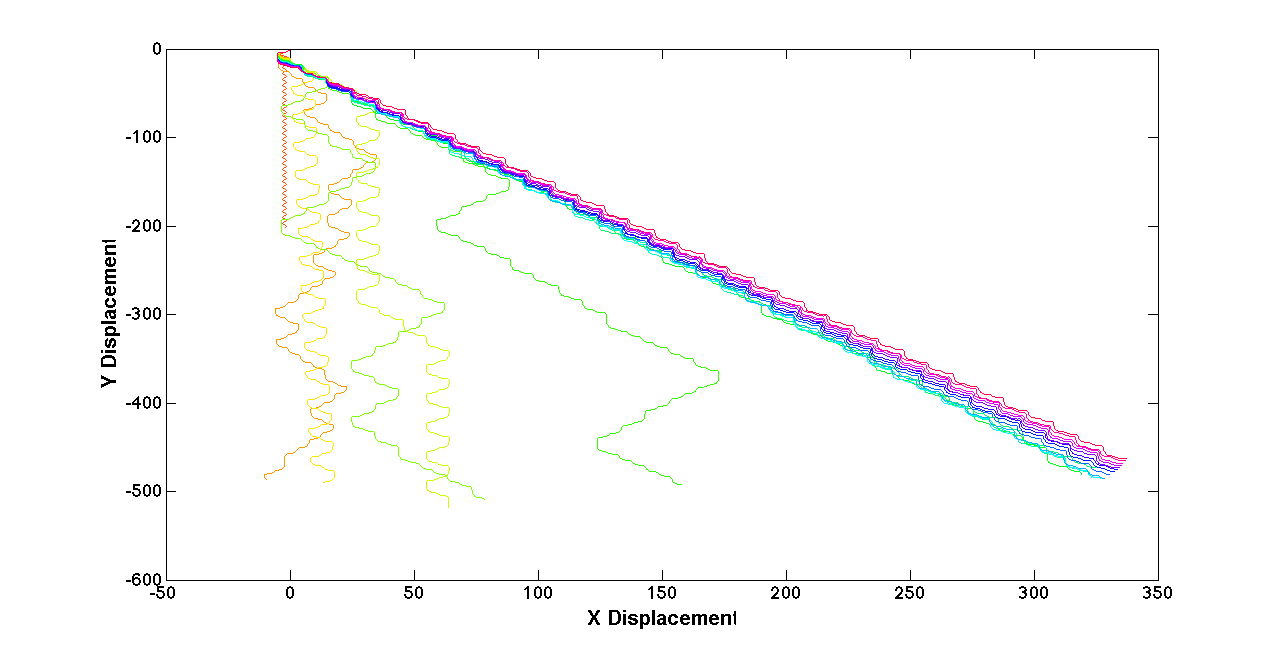
\includegraphics[width=1\linewidth, height=2.5in]{Motion_Graphs/f_xy.png}
	\caption{Plot showing the trajectory of the leaf as the simulation runs, for 20 values of f between 0 and 100. }\label{fig:f_xy}
\end{figure}

\noindent Figure \ref{fig:f_xy} shows the trajectory of the leaf when f is increased. The increase in f means a decrease in the value of $k_{\parallel}$. As $k_{\parallel}$ decreases, the motion of the leaf becomes less oscillatory, and the leaf travels further diagonally. 


\subsection{Length of the Leaf, l}
The length of the leaf can also be varied to get different types of motion. The values chosen are from 0.05 metres to 1 metre.  


\begin{figure}[H]
	\centering
	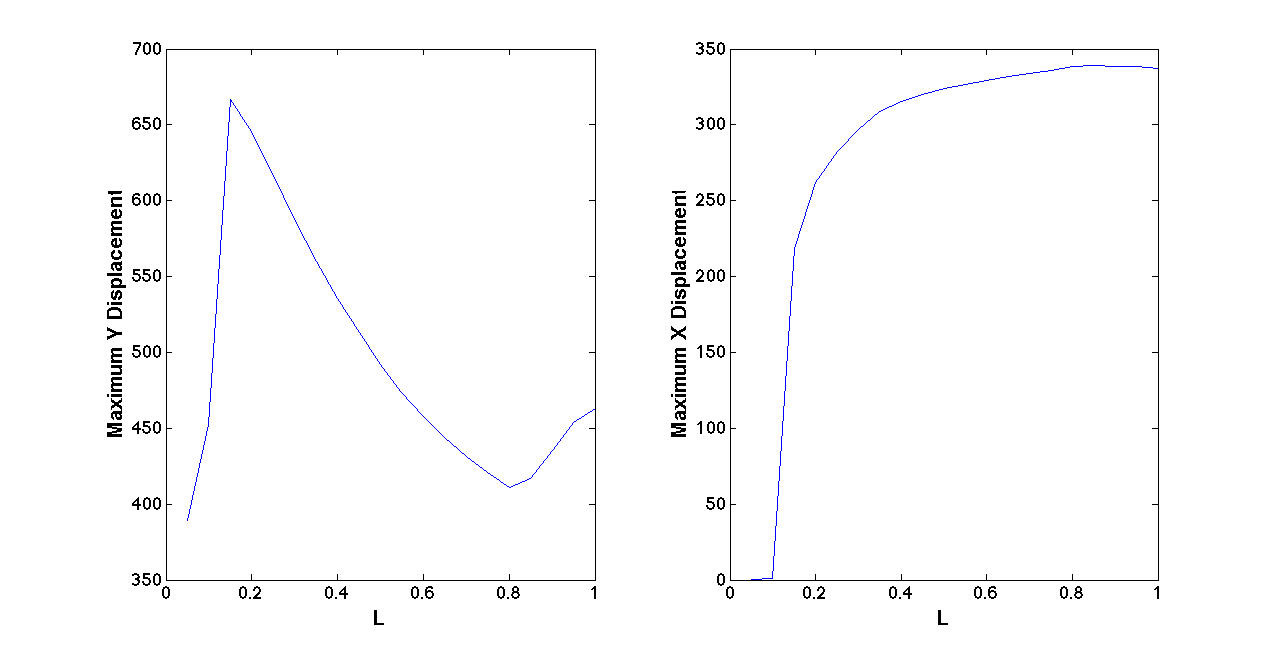
\includegraphics[width=1\textwidth, height=2.5in]{l_max.png}
	\caption{Plot of the maximum $y$ displacement (left) and maximum $x$ displacement (right) against l (the length of the leaf) between 0.05 and 1 metre. }\label{fig:lmax}
\end{figure}

\noindent The left of Figure \ref{fig:lmax} shows the maximum $y$ displacement against the change in l. There is varied behaviour, with the maximum displacement increasing dramatically between 0.05 metres and 0.2 metres, and then decreasing between 0.2 and 0.8. It then begins to increase again around 0.8. 
\newline \newline \noindent The right side shows the change in maximum $x$ displacement, which increases between 0.1 and 0.2, and then levels off at a value of around 340 metres after l reaches 0.3 metres. 

\begin{figure}[H]
	\centering
	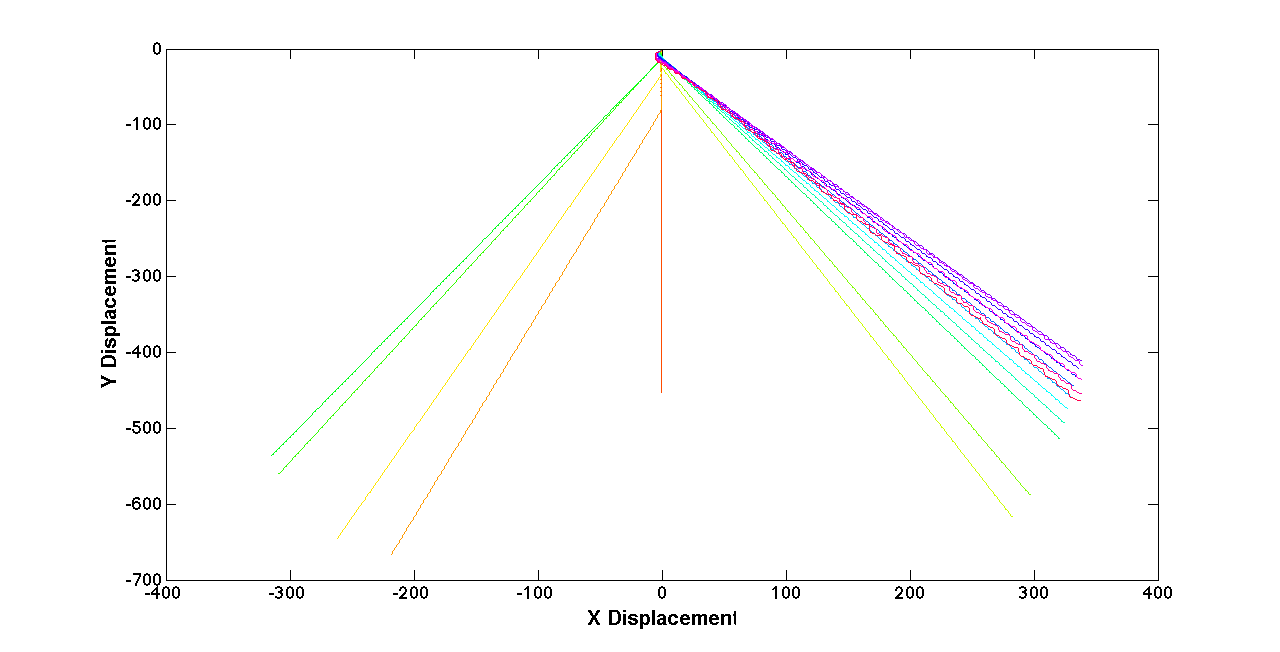
\includegraphics[width=1\linewidth, height=2.5in]{l_xy.png}
	\caption{Plot showing the trajectory of the leaf as the simulation runs for 20 values of l (the length of the leaf) between 0.05 and 1 metre. }\label{fig:l_xy}
\end{figure}


\noindent Figure \ref{fig:l_xy} shows the change of the motion of the leaf as the length is varied. As can be seen from the graph, the change in l does not effect the motion of the leaf greatly, apart from the orange line in the centre for $l = 0.05$.

\begin{figure}[H]
	\centering
	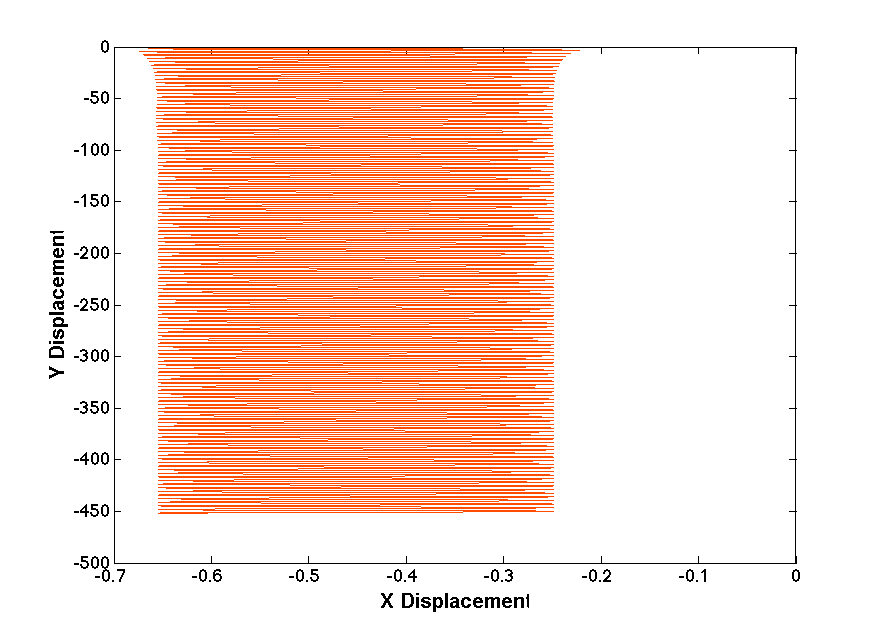
\includegraphics[width=0.7\linewidth, height=2.5in]{Lorange.png}
	\caption{Plot showing the trajectory of the leaf as the simulation runs, for l = 0.05. }\label{fig:lorange}
\end{figure}

\noindent Figure \ref{fig:lorange} shows what looks like a vertical line in Figure \ref{fig:l_xy}, but what is actually small oscillations in the $x$ direction, all of the same value. This type of behaviour only occurs for a value of $l = 0.05$. 

\subsection{Discussion of Parameter Choices}

It is possible to see that the parameters affect the results of the simulations in many different ways. The choice of parameters is influenced by slow motion video footage captured of a piece of paper falling, to allow for the most realistic motion to be simulated.\newline

%what value for kper
\noindent $k_{\perp}$, when increased, causes the displacements in both $x$ and $y$ directions to decrease. In order to choose the best value for this parameter, the video files and simulation graphs were consulted, and the region of values with the best results was chosen to be between 4.5 and 5, at the last point in Figure \ref{fig:kpermax} before the decrease to a constant value in the $y$ direction, and the peak in the $x$ direction.\newline 

%what value for rho
\noindent The value for $\rho$, the ratio of density between the air and the leaf, is a value that can be set as a single constant and ignored thereafter. This is because, once the parameter reaches a certain value, the maximum $x$ and $y$ displacement remain constant. As this is the case, the value of 0.1 for $\rho$ was chosen, as it is at the point where both the maximum $x$ and $y$ displacements begin to level out to constant values. \newline
%what value for f

\noindent The value used for f is also able to be set to a constant, with the choice being a value of 100. This value is chosen because the maximum $x$ and $y$ displacements in Figure \ref{fig:fmax} level out at around this value, and they give believable results for the initial conditions that they are tested with, in comparison with the video footage. \newline

%what value for l

\noindent The difficulty in choosing a value for l, the length of the leaf, lies in two places, whether to look for realistic movement, or a realistic value. The choice sways more in favour of realistic behaviour, because in the case of graphical simulation, realistic behaviour is more important than a true value. As such, a leaf of length 1 metre was chosen, as it gives the best variation of results when initiated with different conditions. 



